% $Id: intro.tex 7102 2008-07-04 14:18:03Z alexandra $
% Local Variables:
% ispell-check-comments: nil
% Local IspellDict: american
% End:
% --------------------------------------------------------
% User documentation
% copyright by BREDEX GmbH 2005
% --------------------------------------------------------
% this command can be inserted multiple times
%\gdhelpid{}
% 
%\begin{gddescription}
%\end{gddescription}
%
%\begin{gdlist}
% use the \item command for single steps
%\end{gdlist}
% change <PATH> to the same directory, file is located in
% change <FILE> to the same filename you are editing
%\bxinput{<PATH>/Links/<FILE>}
%
% other usefull commands are
%   \bxtipp{}        to create a hint
%   \bxwarn{}        to describe a warning
\index{View!Problem}
\index{Problem View}
\index{Error Messages}
\index{Information Messages}
\index{Warning Messages}
\index{Messages!Error}
\index{Messages!Information}
\index{Messages!Warning}
The \gdprobview{} (\bxfigref{probview}) is in the middle of the specification perspective, at the bottom, by default. 

It shows three types of message: 
\begin{itemize}
\item Information
\gdmarpar{../../../share/PS/info}{information}
\item Errors
\gdmarpar{../../../share/PS/error}{error}
\item Warnings
\gdmarpar{../../../share/PS/warning}{warning}
\end{itemize}


Right-clicking on a message and selecting \bxname{Quick Fix} will either solve the problem or take you to the place where you can solve the problem, if this is possible.


\begin{figure}[h]
\begin{center}
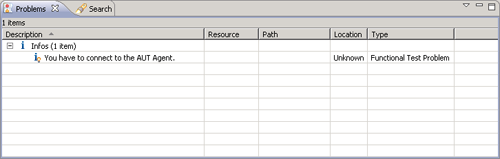
\includegraphics{Tasks/Problemview/PS/probview}
\caption{\gdprobview}
\label{probview}
\end{center}
\end{figure}

%% You can filter the information in the \gdprobview{} by clicking the arrow button in the upper right-hand side of the view and selecting \bxcaption{Preferences}. 

%% In the dialog that appears, you can set the amount of messages of each type to be shown. 

